% wage growth vs int prob figure
\begin{figure}
  \caption{Income distribution across sample sub-groups} \centering
  \label{fig:wageeffect}
  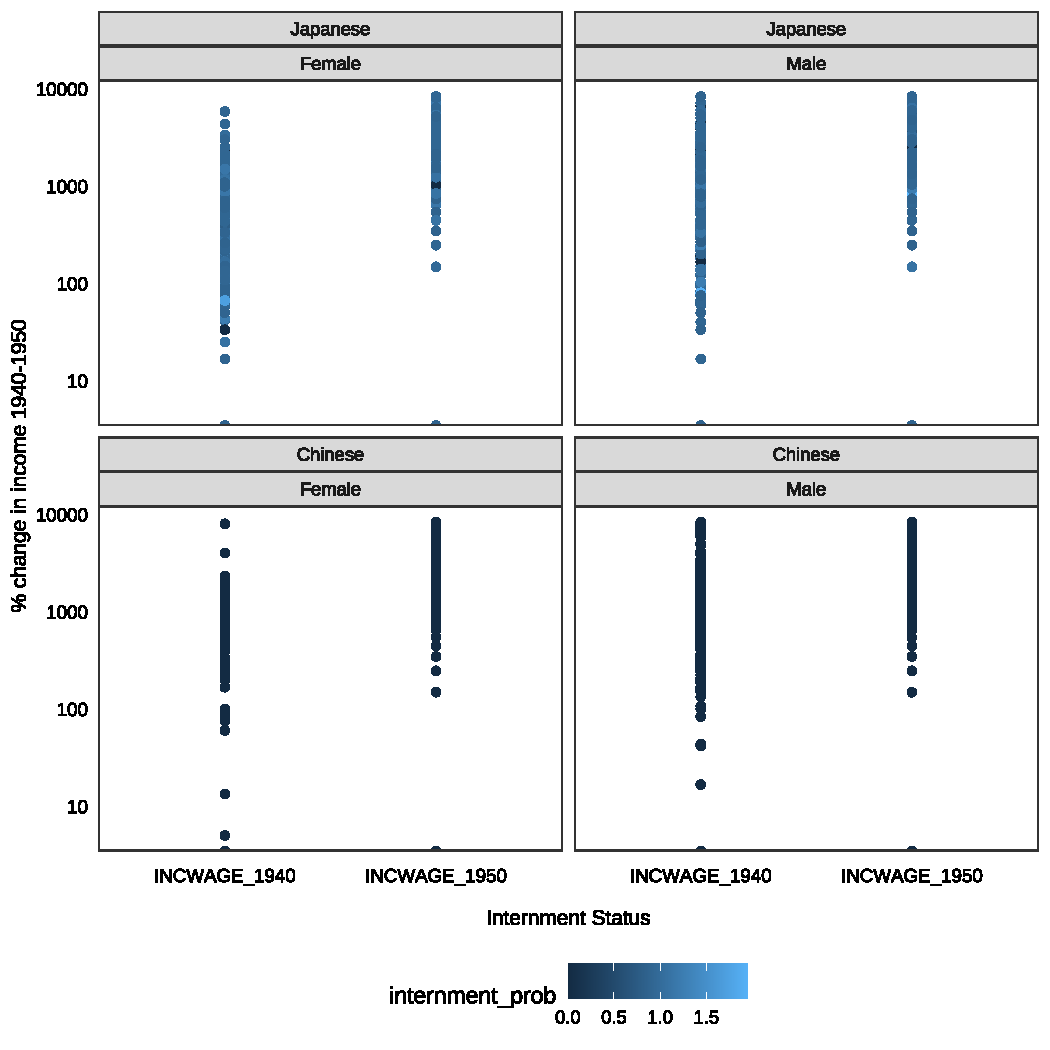
\includegraphics[width=\textwidth]{../figures/INCWAGE_plot.pdf} \\
  \footnotesize
    \emph{Note:}
  Interned proportions are calculated as the number of internees from the county divided by the county's Japanese population in the 1940 full-count census.
  Counties in white had zero Japanese respondents in the 1940 census.
  The map on the below comes from the 1942 Western Defense Command's Final Report 
  % \citep{dewittjohnl.FinalReportJapanese1943}
  and shows in color the evacuation areas along the West Coast.
\end{figure}
